\chapter{Times and Places}\label{times-and-places}

The previous chapter introduces variables and two kinds of values:
integers and floating-point numbers. This chapter presents these
additional types:

\begin{itemize}
\item
  Strings, which represent text.
\item
  Time stamps, which represent dates and times.
\item
  And several ways to represent and display geographical locations.
\end{itemize}

Not every data science project uses all of these types, but many
projects use at least one.

\section{Strings}\label{strings}

A \textbf{string} is a sequence of letters, numbers, and punctuation
marks. In Python you can create a string by enclosing text between
single or double quotation marks.

\begin{lstlisting}[language=Python,style=source]
'Elements'
\end{lstlisting}

\begin{lstlisting}[style=output]
'Elements'
\end{lstlisting}

\begin{lstlisting}[language=Python,style=source]
"of"
\end{lstlisting}

\begin{lstlisting}[style=output]
'of'
\end{lstlisting}

And you can assign string values to variables.

\begin{lstlisting}[language=Python,style=source]
first = 'Data'
last = "Science"
\end{lstlisting}

Some arithmetic operators work with strings, but they might not do what
you expect. For example, the \passthrough{\lstinline!+!} operator
\textbf{concatenates} two strings -- that is, it creates a new string
that contains the first string followed by the second string:

\begin{lstlisting}[language=Python,style=source]
first + last
\end{lstlisting}

\begin{lstlisting}[style=output]
'DataScience'
\end{lstlisting}

If you want to put a space between the words, you can use a string that
contains a space:

\begin{lstlisting}[language=Python,style=source]
first + ' ' + last
\end{lstlisting}

\begin{lstlisting}[style=output]
'Data Science'
\end{lstlisting}

Strings are used to store text data like names, addresses, titles, etc.
When you read data from a file, you might see values that look like
numbers, but they are actually strings, like this:

\begin{lstlisting}[language=Python,style=source]
not_actually_a_number = '123'
\end{lstlisting}

If you try to do math with these strings, you \emph{might} get an error.

\begin{lstlisting}[language=Python,style=source]
%%expect TypeError

not_actually_a_number + 1
\end{lstlisting}

\begin{lstlisting}[style=output]
TypeError: can only concatenate str (not "int") to str
\end{lstlisting}

But you might not -- instead, you might get a surprising result. For
example:

\begin{lstlisting}[language=Python,style=source]
not_actually_a_number * 3
\end{lstlisting}

\begin{lstlisting}[style=output]
'123123123'
\end{lstlisting}

If you multiply a string by an integer, Python repeats the string the
given number of times.

If you have a string that contains only digits, you can convert it to an
integer using the \passthrough{\lstinline!int!} function:

\begin{lstlisting}[language=Python,style=source]
int('123')
\end{lstlisting}

\begin{lstlisting}[style=output]
123
\end{lstlisting}

\pagebreak

Or you can convert it to a floating-point number using
\passthrough{\lstinline!float!}:

\begin{lstlisting}[language=Python,style=source]
float('12.3')
\end{lstlisting}

\begin{lstlisting}[style=output]
12.3
\end{lstlisting}

But if the string contains a decimal point, you can't convert it to an
\passthrough{\lstinline!int!}.

\begin{lstlisting}[language=Python,style=source]
%%expect ValueError

int('12.3')
\end{lstlisting}

\begin{lstlisting}[style=output]
ValueError: invalid literal for int() with base 10: '12.3'
\end{lstlisting}

Going in the other direction, you can convert any type of value to a
string using \passthrough{\lstinline!str!}:

\begin{lstlisting}[language=Python,style=source]
str(123)
\end{lstlisting}

\begin{lstlisting}[style=output]
'123'
\end{lstlisting}

\begin{lstlisting}[language=Python,style=source]
str(12.3)
\end{lstlisting}

\begin{lstlisting}[style=output]
'12.3'
\end{lstlisting}

\textbf{Exercise}: When personal names are stored in a database, they
might be stored in variables representing one or more given names,
family names, and maybe additional middle names. For example, a list of
early statisticians might include:

\begin{lstlisting}[language=Python,style=source]
given = 'William'
middle = 'Sealy'
family = 'Gosset'
\end{lstlisting}

But names are often displayed different ways in different contexts. For
example, the first time you mention someone in a book, you might give
all three names, like ``William Sealy Gosset''. But in the index, you
might put the family name first, like ``Gosset, William Sealy''. Write
Python expressions that use the variables
\passthrough{\lstinline!given!}, \passthrough{\lstinline!middle!}, and
\passthrough{\lstinline!family!} to display Gosset's name in these two
formats.

\section{Representing Dates and
Times}\label{representing-dates-and-times}

When you read data from a file, you might find that dates and times are
represented with strings.

\begin{lstlisting}[language=Python,style=source]
not_really_a_date = 'June 4, 1989'
\end{lstlisting}

\pagebreak

To check the type of a value, we can use the
\passthrough{\lstinline!type!} function.

\begin{lstlisting}[language=Python,style=source]
type(not_really_a_date)
\end{lstlisting}

\begin{lstlisting}[style=output]
str
\end{lstlisting}

The result indicates that the value of
\passthrough{\lstinline!not\_really\_a\_date!} is a string.

We get the same result with
\passthrough{\lstinline!not\_really\_a\_time!}, below:

\begin{lstlisting}[language=Python,style=source]
not_really_a_time = '6:30:00'
type(not_really_a_time)
\end{lstlisting}

\begin{lstlisting}[style=output]
str
\end{lstlisting}

Strings that represent dates and times are readable for people, but they
are not useful for computation. Fortunately, Python provides libraries
for working with date and time data -- the one we'll use is called
Pandas. As always, we have to import a library before we use it. It is
conventional to import Pandas with the abbreviated name
\passthrough{\lstinline!pd!}:

\begin{lstlisting}[language=Python,style=source]
import pandas as pd
\end{lstlisting}

Pandas provides a type called \passthrough{\lstinline!Timestamp!}, which
represents a date and time. If we have a string that contains a time or
date, we can convert it to a \passthrough{\lstinline!Timestamp!} like
this:

\begin{lstlisting}[language=Python,style=source]
pd.Timestamp('6:30:00')
\end{lstlisting}

\begin{lstlisting}[style=output]
Timestamp('2024-05-18 06:30:00')
\end{lstlisting}

Or we can do the same thing using the variable defined above.

\begin{lstlisting}[language=Python,style=source]
pd.Timestamp(not_really_a_time)
\end{lstlisting}

\begin{lstlisting}[style=output]
Timestamp('2024-05-18 06:30:00')
\end{lstlisting}

In this example, the string specifies a time but no date, so Pandas
fills in today's date. A \passthrough{\lstinline!Timestamp!} is a value,
so you can assign it to a variable.

\begin{lstlisting}[language=Python,style=source]
date_of_birth = pd.Timestamp('May 11, 1967')
date_of_birth
\end{lstlisting}

\begin{lstlisting}[style=output]
Timestamp('1967-05-11 00:00:00')
\end{lstlisting}

If the string specifies a date but no time, Pandas fills in midnight as
the default time.

\pagebreak

If you assign the \passthrough{\lstinline!Timestamp!} to a variable, you
can use the variable name to get the year, month, and day, like this:

\begin{lstlisting}[language=Python,style=source]
date_of_birth.year, date_of_birth.month, date_of_birth.day
\end{lstlisting}

\begin{lstlisting}[style=output]
(1967, 5, 11)
\end{lstlisting}

You can also get the name of the month and the day of the week.

\begin{lstlisting}[language=Python,style=source]
date_of_birth.day_name(), date_of_birth.month_name()
\end{lstlisting}

\begin{lstlisting}[style=output]
('Thursday', 'May')
\end{lstlisting}

\passthrough{\lstinline!Timestamp!} provides a function called
\passthrough{\lstinline!now!} that returns the current date and time.

\begin{lstlisting}[language=Python,style=source]
now = pd.Timestamp.now()
now
\end{lstlisting}

\begin{lstlisting}[style=output]
Timestamp('2024-05-18 15:04:03.507085')
\end{lstlisting}

\textbf{Exercise:} Use the value of \passthrough{\lstinline!now!} to
display the name of the current month and day of the week.

\section{Timedelta}\label{timedelta}

\passthrough{\lstinline!Timestamp!} values support some arithmetic
operations. For example, you can compute the difference between two
\passthrough{\lstinline!Timestamp!} objects:

\begin{lstlisting}[language=Python,style=source]
age = now - date_of_birth
age
\end{lstlisting}

\begin{lstlisting}[style=output]
Timedelta('20827 days 15:04:03.507085')
\end{lstlisting}

The result is a \passthrough{\lstinline!Timedelta!} that represents the
current age of someone born on
\passthrough{\lstinline!date\_of\_birth!}. The
\passthrough{\lstinline!Timedelta!} contains
\passthrough{\lstinline!components!} that store the number of days,
hours, etc. between the two \passthrough{\lstinline!Timestamp!} values.

\begin{lstlisting}[language=Python,style=source]
from utils import wrap

wrap(age.components)
\end{lstlisting}

\begin{lstlisting}[style=output]
Components(days=20827, hours=15, minutes=4, seconds=3,
    milliseconds=507, microseconds=85, nanoseconds=0)
\end{lstlisting}

\pagebreak

You can get one of the components like this:

\begin{lstlisting}[language=Python,style=source]
age.days
\end{lstlisting}

\begin{lstlisting}[style=output]
20827
\end{lstlisting}

It might seem strange to measure a large interval in days rather than
years. The problem is that the duration of a year is not clearly
defined. Most years are \passthrough{\lstinline!365!} days, but some are
\passthrough{\lstinline!366!}. The average calendar year is
\passthrough{\lstinline!365.24!} days, which is a very good
approximation of a solar year, but even that's not exact.

Expressing a duration in days is clearly defined -- but it is not easy
to interpret. To express \passthrough{\lstinline!age!} in years, we can
divide by \passthrough{\lstinline!365.24!}:

\begin{lstlisting}[language=Python,style=source]
age.days / 365.24
\end{lstlisting}

\begin{lstlisting}[style=output]
57.022779542218814
\end{lstlisting}

But people usually report their ages in integer years. We can use the
Numpy \passthrough{\lstinline!floor!} function to round down:

\begin{lstlisting}[language=Python,style=source]
import numpy as np

np.floor(age.days / 365.24)
\end{lstlisting}

\begin{lstlisting}[style=output]
57.0
\end{lstlisting}

Or the \passthrough{\lstinline!ceil!} function (which stands for
``ceiling'') to round up:

\begin{lstlisting}[language=Python,style=source]
np.ceil(age.days / 365.24)
\end{lstlisting}

\begin{lstlisting}[style=output]
58.0
\end{lstlisting}

We can also compare \passthrough{\lstinline!Timestamp!} values to see
which comes first. For example, let's see if a person with a given
birthdate has already had a birthday this year. Here's a new
\passthrough{\lstinline!Timestamp!} with the year from
\passthrough{\lstinline!now!} and the month and day from
\passthrough{\lstinline!date\_of\_birth!}.

\begin{lstlisting}[language=Python,style=source]
bday_this_year = pd.Timestamp(now.year,
                              date_of_birth.month,
                              date_of_birth.day)
bday_this_year
\end{lstlisting}

\begin{lstlisting}[style=output]
Timestamp('2024-05-11 00:00:00')
\end{lstlisting}

The result represents the person's birthday this year.

\pagebreak

Now we can use
the ``greater than'' operator, \passthrough{\lstinline!>!}, to check
whether \passthrough{\lstinline!now!} is later than the birthday:

\begin{lstlisting}[language=Python,style=source]
now > bday_this_year
\end{lstlisting}

\begin{lstlisting}[style=output]
True
\end{lstlisting}

The result is either \passthrough{\lstinline!True!} or
\passthrough{\lstinline!False!}. These values belong to a type called
\passthrough{\lstinline!bool!}. The name comes from ``Boolean algebra'',
which is a branch of algebra where all values are either true or false.

\begin{lstlisting}[language=Python,style=source]
type(True)
\end{lstlisting}

\begin{lstlisting}[style=output]
bool
\end{lstlisting}

\begin{lstlisting}[language=Python,style=source]
type(False)
\end{lstlisting}

\begin{lstlisting}[style=output]
bool
\end{lstlisting}

\textbf{Exercise:} Any two people with different birthdays have a
``Double Day'' when one is twice as old as the other. Suppose you are
given two \passthrough{\lstinline!Timestamp!} values,
\passthrough{\lstinline!d1!} and \passthrough{\lstinline!d2!}, that
represent birthdays for two people. Use
\passthrough{\lstinline!Timestamp!} arithmetic to compute their double
day. With the following dates, the result should be December 19, 2009.

\begin{lstlisting}[language=Python,style=source]
d1 = pd.Timestamp('2003-07-12')
d2 = pd.Timestamp('2006-09-30')
\end{lstlisting}

\section{Representing Location}\label{representing-location}

In addition to times and dates, we might also want to represent
locations, especially if we are working with geographical data. There
are many ways to represent locations, but the most common, at least for
global data, is latitude and longitude. When stored in a string,
latitude and longitude are expressed in degrees with compass directions
N, S, E, and W. For example, this string represents the location of
Boston, Massachusetts, USA:

\begin{lstlisting}[language=Python,style=source]
lat_lon_string = '42.3601° N, 71.0589° W'
\end{lstlisting}

But for purposes of computation it is more common to represent longitude
and latitude with two floating-point numbers, with

\begin{itemize}
\item
  Positive latitude for locations in the northern hemisphere, negative
  latitude for the southern hemisphere, and
\item
  Positive longitude locations in the eastern hemisphere and negative
  longitude for the western hemisphere.
\end{itemize}

The location of the origin and the orientation of positive and negative
are arbitrary choices that were made for historical reasons.

\pagebreak

Here's how
we might represent the location of Boston with two variables.

\begin{lstlisting}[language=Python,style=source]
lat = 42.3601
lon = -71.0589
\end{lstlisting}

It is also possible to combine two numbers into a composite value and
assign it to a single variable:

\begin{lstlisting}[language=Python,style=source]
boston = lat, lon
boston
\end{lstlisting}

\begin{lstlisting}[style=output]
(42.3601, -71.0589)
\end{lstlisting}

The type of this variable is \passthrough{\lstinline!tuple!}, which is a
mathematical term for a value that contains a sequence of elements. Math
people pronounce it ``tuh' ple'', but computational people usually say
``too' ple''. Either is fine.

\begin{lstlisting}[language=Python,style=source]
type(boston)
\end{lstlisting}

\begin{lstlisting}[style=output]
tuple
\end{lstlisting}

If you have a tuple with two elements, you can assign them to two
variables, like this:

\begin{lstlisting}[language=Python,style=source]
y, x = boston
y
\end{lstlisting}

\begin{lstlisting}[style=output]
42.3601
\end{lstlisting}

\begin{lstlisting}[language=Python,style=source]
x
\end{lstlisting}

\begin{lstlisting}[style=output]
-71.0589
\end{lstlisting}

Notice that I assigned latitude to \passthrough{\lstinline!y!} and
longitude to \passthrough{\lstinline!x!}, because a
\passthrough{\lstinline!y!} coordinate usually goes up and down like
latitude, and an \passthrough{\lstinline!x!} coordinate usually goes
side-to-side like longitude.

\textbf{Exercise:} Find the latitude and longitude of the place you were
born or someplace you think of as your ``home town''. Make a tuple of
floating-point numbers that represents that location.

\section{Calculating Distance}\label{calculating-distance}

If you are given two tuples that represent locations, you can compute
the approximate distance between them, along the surface of the globe,
using the haversine function:

\(\mathrm{haversine}(\theta)=\sin^2(\theta/2)\)

where \(\theta\) is an angle in radians.

\pagebreak

We can compute this function in
Python like this:

\begin{lstlisting}[language=Python,style=source]
import numpy as np

θ = 1
np.sin(θ/2)**2
\end{lstlisting}

\begin{lstlisting}[style=output]
0.22984884706593015
\end{lstlisting}

You can use Greek letters in variable names, but there is currently no
way to type them in Jupyter/Colab, so I usually copy them from a web
page and paste them in. To avoid the inconvenience, it is common to
write out letter names, like this:

\begin{lstlisting}[language=Python,style=source]
theta = 1
np.sin(theta/2)**2
\end{lstlisting}

\begin{lstlisting}[style=output]
0.22984884706593015
\end{lstlisting}

Remember that the operator for exponentiation is
\passthrough{\lstinline!**!}. In some other languages it's
\passthrough{\lstinline!\^!}, which is also an operator in Python, but
it performs another operation altogether.

\section{Defining Functions}\label{defining-functions}

If we are planning to use an expression like
\passthrough{\lstinline!np.sin(theta/2)**2!} more than a few times, we
can define a new function that computes it, like this:

\begin{lstlisting}[language=Python,style=source]
def haversine(theta):
    """Compute the haversine function of theta."""
    return np.sin(theta/2)**2
\end{lstlisting}

On the first line, \passthrough{\lstinline!def!} indicates that we are
defining a function. The second line is a triple-quoted string, which is
a \textbf{comment}: it describes what the function does, but has no
effect when the program runs. On the third line,
\passthrough{\lstinline!return!} indicates the result of the function.

When you run the previous cell, it creates a new variable called
\passthrough{\lstinline!haversine!}. You can display its value like
this:

\begin{lstlisting}[language=Python,style=source]
haversine
\end{lstlisting}

\begin{lstlisting}[style=output]
<function __main__.haversine(theta)>
\end{lstlisting}

And you can display its type like this:

\begin{lstlisting}[language=Python,style=source]
type(haversine)
\end{lstlisting}

\begin{lstlisting}[style=output]
function
\end{lstlisting}

So \passthrough{\lstinline!haversine!} is a variable that refers to a
function. To run the function and compute a result, we have to
\textbf{call} the function and provide a value for
\passthrough{\lstinline!theta!}:

\begin{lstlisting}[language=Python,style=source]
haversine(1)
\end{lstlisting}

\begin{lstlisting}[style=output]
0.22984884706593015
\end{lstlisting}

When you define a function, you create a new variable. But the function
doesn't actually run until you call it.

\section{Haversine Distance}\label{haversine-distance}

Now we can use \passthrough{\lstinline!haversine!} as part of a function
that computes haversine distances. I won't explain this function in as
much detail, but if you read through it, you can get a sense of how it
works.

\begin{lstlisting}[language=Python,style=source]
def haversine_distance(coord1, coord2):
    """Haversine distance between two locations.

    coord1: lat-lon as tuple of float
    coord2: lat-lon as tuple of float

    returns: distance in km
    """
    R = 6372.8  # Earth radius in km
    lat1, lon1 = coord1
    lat2, lon2 = coord2

    phi1, phi2 = np.radians(lat1), np.radians(lat2)
    dphi = np.radians(lat2 - lat1)
    dlambda = np.radians(lon2 - lon1)

    a = haversine(dphi) + np.cos(phi1) * np.cos(phi2) * haversine(dlambda)

    distance = 2 * R * np.arctan2(np.sqrt(a), np.sqrt(1 - a))

    return distance
\end{lstlisting}

When we call this function, we provide two tuples; each is a
latitude-longitude pair. We already have a tuple that represents the
location of Boston. Now here's a tuple that represents the location of
London, England, UK:

\begin{lstlisting}[language=Python,style=source]
london = 51.5074, -0.1278
\end{lstlisting}

\pagebreak

And here's the haversine distance between Boston and London.

\begin{lstlisting}[language=Python,style=source]
haversine_distance(boston, london)
\end{lstlisting}

\begin{lstlisting}[style=output]
5265.656325981015
\end{lstlisting}

The actual geographic distance is slightly different because Earth is
not a perfect sphere. But the error of this estimate is less than 1\%.

\textbf{Exercise:} Use \passthrough{\lstinline!haversine\_distance!} to
compute the distance between Boston and your home town from the previous
exercise. If possible, use an online map to check the result.

\section{Geopandas}\label{geopandas}

Python provides libraries for working with geographical data. One of the
most popular is Geopandas, which is based on Pandas and another library
called Shapely. Shapely provides \passthrough{\lstinline!Point!} and
\passthrough{\lstinline!LineString!} values, which we'll use to
represent geographic locations and lines between them.

\begin{lstlisting}[language=Python,style=source]
from shapely.geometry import Point, LineString
\end{lstlisting}

We can use the tuples we defined in the previous section to create
Shapely \passthrough{\lstinline!Point!} values, but we have to reverse
the order of the coordinates, providing them in
\passthrough{\lstinline!x!}-\passthrough{\lstinline!y!} order rather
than \passthrough{\lstinline!lat!}-\passthrough{\lstinline!lon!} order,
because that's the order the \passthrough{\lstinline!Point!} function
expects.

\begin{lstlisting}[language=Python,style=source]
lat, lon = boston
p1 = Point(lon, lat)
\end{lstlisting}

\begin{lstlisting}[language=Python,style=source]
lat, lon = london
p2 = Point(lon, lat)
\end{lstlisting}

We can use the points we just defined to create a
\passthrough{\lstinline!LineString!}:

\begin{lstlisting}[language=Python,style=source]
line = LineString([p1, p2])
\end{lstlisting}

Now we can use Geopandas to show these points and lines on a map. The
following cells load a map of the world and plot it.

\begin{lstlisting}[language=Python,style=source]
from geodatasets import fetch

fetch('naturalearth.land')
\end{lstlisting}

\begin{lstlisting}[language=Python,style=source]
from geodatasets import get_path

path = get_path('naturalearth.land')
\end{lstlisting}

\begin{lstlisting}[language=Python,style=source]
import geopandas as gpd
world = gpd.read_file(path)
world.plot(color='white', edgecolor='gray');
\end{lstlisting}

\begin{center}
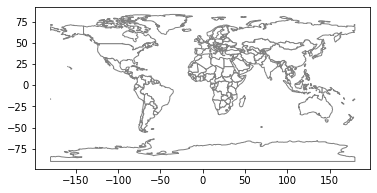
\includegraphics[scale=0.6666666]{02_times_files/02_times_127_0.png}
\end{center}

By default, Geopandas uses an equirectangular projection, which provides
a misleading picture of relative land areas. Other projections are
available that show land areas accurately, but they can be misleading in
other ways. You can't make a map without making visualization decisions.

Now let's put dots on the map for Boston and London. First, we have to
put the \passthrough{\lstinline!Point!} values and the
\passthrough{\lstinline!LineString!} into a
\passthrough{\lstinline!GeoSeries!}.

\begin{lstlisting}[language=Python,style=source]
t = [p1, p2, line]
series = gpd.GeoSeries(t)
\end{lstlisting}

Here's a first attempt to plot the maps and the lines together:

\begin{lstlisting}[language=Python,style=source]
# plot the map
world.plot(color='white', edgecolor='gray')

# plot Boston, London, and the line
series.plot();
\end{lstlisting}

\begin{center}
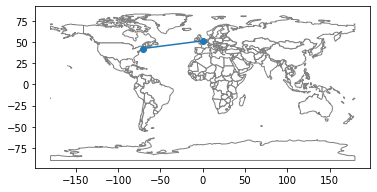
\includegraphics[scale=0.6666666]{02_times_files/02_times_131_0.png}
\end{center}

\begin{center}
\includegraphics[scale=0.6666666]{02_times_files/02_times_131_1.png}
\end{center}

The two plots are on different axes, which is not what we want in this
case.

To get the points and the map on the same axes, we have to use a
function from Matplotlib, which is a visualization library we will use
extensively. We'll import it like this.

\begin{lstlisting}[language=Python,style=source]
import matplotlib.pyplot as plt
\end{lstlisting}

From Matplotlib, we'll use the function \passthrough{\lstinline!gca!},
which stands for ``get current axes''. With the result we can tell
\passthrough{\lstinline!plot!} to put the points and lines on the
current axes, rather than create a new one.

\begin{lstlisting}[language=Python,style=source]
ax = plt.gca()
world.plot(color='white', edgecolor='gray', ax=ax)
series.plot(ax=ax);
\end{lstlisting}

\begin{center}
\includegraphics[scale=0.6666666]{02_times_files/02_times_135_0.png}
\end{center}

\textbf{Exercise:} Modify the code in this section to plot a point that
shows the home town you chose in a previous exercise and a line from
there to Boston.

\section{Summary}\label{summary}

This chapter presents three new data types: strings to represent letters
and words, \passthrough{\lstinline!Timestamp!} objects to represent
dates and times, and tuples to represent latitude, longitude pairs. It
also introduces Geopandas, a library for working with location data.

In the next chapter we'll see two ways to represent a collection of
data, a Python list and a Numpy array.
